\subsubsection{Evaluation verfügbarer Produkte}
\label{chap:produkt-eval}
\paragraph{Auswahl der \ac{WAF}-Anwendung}

\paragraph{Verwundbare Anwendungen}

\subsubsection{Labor-Umgebung}

% 1. Anforderungen an die Lernumgebung
% 2. Überlegungen zur gestaltung einheiltichen Deployments
% 2.1. Docker
%       - einheitlich
%       - Netzwerke
%       - Probleme mit croscompatibility (Windows)
% 2.2. VM (vortiele und Probleme)
% 3. beschreibung der Container
% 3.1. Juicesop
% 3.2. WAF
% 3.3. Python contaienr mit test script

Die in Kapitel \ref{chap:inhalte} beschriebenen Inhalte sollen in einem Praxisnahen Umfeld vermittelt werden.
Dazu kommt nach den Abwägungen aus Kapitel \ref{chap:produkt-eval}, die Waf-Applikation ModSecurity zum Einsatz.
Die zu diesem Zweck vorgesehene Laborumgebung muss einige Kriterien erfüllen:
\begin{description}
    \item[Einheitliches Deployment:]  Der Ausgangspunkt der Lerneinheiten muss reproduzierbar und wiederholbar sein. Bei wiederholten Durchführungen der Übungen soll es einfach sein den Lernenden ohne zusätzlichen Manuellen Konfigurationsaufwand eine Laborumgebung zu übergeben.
    \item[Modifizierbarketit der Anwendungen:] Um in den Lerneinheiten grundlegende Techniken zu übermitteln, ist es notwendig Basis-Funktionen entfernen zu können. Und die 
    \item[Bekannte Basis-Technologien:]
    \item[Komplexe Netzwerkumgebungen:]
\end{description}

\begin{figure}[!hbt]
    \centering
    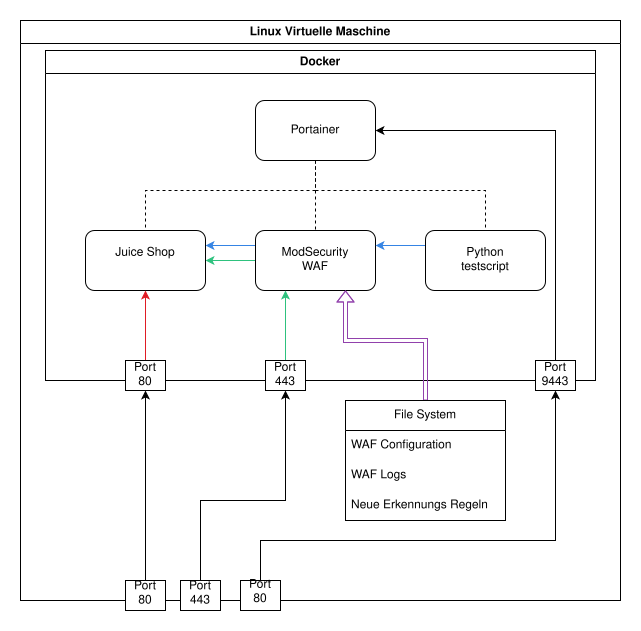
\includegraphics[width=0.9\textwidth]{./images/lab-setup.png}
    \caption{Aufbau der Laborumgebung}
    \label{fig:lab}
\end{figure}

